\section{Passivation}
In most silicates the silicon atoms have tetrahedral coordination, with four oxygen atoms surronding each silicon atom. When we remove silica- and oxygen-atoms to create a fracture, we do not take this into consideration. This means that we get dangling unsaturated bonds in the system, located near the surface of the pore. To rectify this we use a method called passivation, where we saturate and passivate the dangling bonds by inserting new atoms. 

\subsection{Water chemistry}
Since we are going to inject water into the pore later on, we want to use the constituents of water to passivate the system. We know that water autodissociates into H$^{+}$ and OH$^{-}$ via the following reaction
\begin{align*}
    \text{H}_2\text{O} \rightleftharpoons \text{H}^{+} + \text{OH}^{-},
\end{align*}
meaning that hydrogen (H) and hydroxide (OH) will be freely available in the system after filling the pore with water. On this background we choose to passivate the system using hydrogen and hydroxide. To avoid getting an acidic or alkaline system after the passivation procedure we should make sure to use equal parts hydrogen and hydroxide when passivating.

\subsection{Passivating using hydrogen and hydroxide}
After thermalizing our silica system we end up with a system consisting almost exclusively of SiO$_2$ tetrahedra. These tetrahedra are each formed by four oxygen atoms, one in each corner, and a silicon atom in the center. Each of these tetrahedra are then bonded to four other tetrahedra, by sharing the oxygen atoms in the corners. This way each oxygen atom is bonded to two silicon atoms, and each silicon atom to four oxygen atoms, giving an average chemical formula of SiO$_2$. 

Since we do not take chemical bonds into consideration when removing atoms to create a fracture, we end up with some incomplete tetrahedra, with some silicon atoms bonded to less than four oxygen atoms, and some oxygen atoms bonded to less than two silicon atoms. See \cref{fig:passivation} for an illustration of three different incomplete tetrahedra. This creates what we call dangling ends or unsaturated bonds, which we want to passivate.

% When inserting hydrogen and hydroxide we want to insert them in positions that are close to their equilibrium positions, so we do not have to do a lot of simulating to get a stabilized system after passivating. It is possible to calculate the optimal positions based on the potential and the positions of the existing atoms, but this is a complicated computation, that we can avoid, by instead realizing that the optimal positions for the oxygen atoms we insert will most likely \hl{(source?)} be close to the positions that complete the SiO$_2$ tetrahedra. These positions can be calculated, using simple geometry, from the positions of the oxygen atoms each silicon atom is bonded to.

To passivate the silicon atoms that are bonded to less than four oxygen atoms, we see that we need to complete the incomplete SiO$_4$ tetrahedra that have been created in the system. But if we only insert oxygen atoms in the positions of the missing oxygen atoms, we end up with new dangling ends, since the inserted oxygen atoms will only be bonded to one silicon atom. But, as we just saw, we will have hydroxide (OH) groups available in the system after filling the fracture with water. So instead of inserting oxygen atoms and creating new unsaturated bonds, we insert hydroxide groups and create saturated Si-O-H bonds. We put the hydrogen atom so that the Si-O-H angle is close to the angle in water molecules, 107.5 degrees. %\hl{The hydrogen atoms moves very rapidly compared to the rest of the species in the system, so they will quicly find the equilibrium position, meaning that the exact position of the hydrogen atoms is not that important.}

To passivate the oxygen atoms that are bonded to only one silicon atom, we can use the hydrogen atoms that are avilable after filling the fracture with water, turning unsaturated SiO-groups into the same saturated Si-O-H-groups as before. We here too insert the hydrogen atoms with the Si-O-H angle close to 107.5 degrees.

In total we use the following procedure to passivate a system after creating a fracture:
\begin{itemize}
    \item Remove all silicon and oxygen atoms that are not bonded to any atoms, since they are essentially not part of the silica matrix.
    \item Add one hydrogen atom to all oxygen atoms bonded to only one silicon atom. The hydrogen atoms are inserted approximately $0.95\text{ \AA}$ from the oxygen atoms, with the hydrogen atom pointing away from the silicon atom, and with the Si-O-H angle close to 107.5 degrees.
    \item Add ($4-n$) hydroxide groups to silicon atoms bonded to $(1\leq n<4)$ oxygen atoms. We assume that the most stable position for the oxygen in the hydroxide groups are close to the tetrahedral positions of the missing oxygen atoms, and insert the hydroxide groups in these positions. %
    %See \cref{fig:pass_tet01,fig:pass_tet02,fig:pass_tet03} for the three different cases. 
    The hydroxide groups are inserted approximately $1.65\text{ \AA}$ from the silicon atoms, measured from the position of the silicon atom to the oxygen atom in the hydroxide groups, with the hydrogen atom pointing away from the silicon atom, and with the Si-O-H angle close to 107.5 degrees.
\end{itemize}
The lengths used are approximate experimental lengths found in naturally occuring silanols and water (see \cite{lickiss1995synthesis} for the Si-O length in silanol, and \cite{csaszar2005equilibrium} for the O-H length in water). This procedure turns all dangling ends into stable, passive silanol groups.
%
\begin{figure}[htpb]%
    \centering%
    \setlength{\myfigwidth}{0.17\textwidth}
    \begin{subfigure}[c]{0.8\myfigwidth}%
        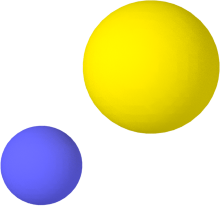
\includegraphics[width=\textwidth]{images/passivation/tetrahedra01_01.png}%
        \caption{}%
%         \caption{Illustration of how to divide a convex hexahedron into five tetraheda.}%
        \label{fig:pass_tet01}%
    \end{subfigure}%
    \hspace{1cm}%
    \begin{subfigure}[c]{\myfigwidth}%
        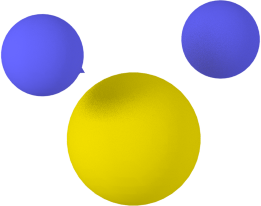
\includegraphics[width=\textwidth]{images/passivation/tetrahedra02_01.png}%
        \caption{}%
%         \caption{A random fracture made from two periodic heightmaps.}%
        \label{fig:pass_tet02}%
    \end{subfigure}%
    \hspace{1cm}%
    \begin{subfigure}[c]{1.1\myfigwidth}%
        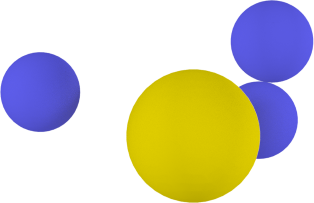
\includegraphics[width=\textwidth]{images/passivation/tetrahedra03_01.png}%
        \caption{}%
%         \caption{A random fracture made from two periodic heightmaps.}%
        \label{fig:pass_tet03}%
    \end{subfigure}%
    \hspace{1cm}%
    \begin{subfigure}[c]{1.1\myfigwidth}%
        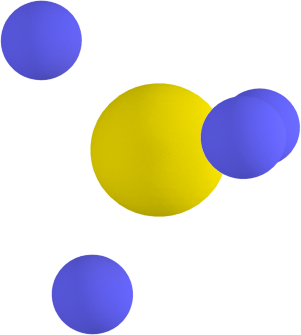
\includegraphics[width=\textwidth]{images/passivation/tetrahedra04_01.png}%
        \caption{}%
%         \caption{A random fracture made from two periodic heightmaps.}%
%         \label{fig:fracture_model}\caption{}%
    \end{subfigure}%
    \caption{%
        Illustration of four different incomplete silica tetrahedra, with respectively one, two, three and no missing oxygen atoms (\textbf{(d)} is a complete silica tetrahedra).%
    }%
    \label{fig:passivation}%
\end{figure}%

\subsection{Counting number of bonds}
Since we do not have actual bonds in molecular dynamics simulations, we do not know which atoms are bonded to which. So to find the number of bonded atoms for each silicon and oxygen atom, we create what we call \emph{neigbor lists}. These neighbor lists are a list of atoms within a chosen radius for each atom. To create these lists we use the procedure detailed in \cref{sec:neighbor_lists}. Since we only have silicon and oxygen atoms in our system, we only need to specify a maximum the Si-O-distance to find which atoms are bonded. If we choose this distance properly, we should be able find a good approximation to how many atoms each atom is bonded to.%
\todobo{Something about g(r) for deciding Si-O bond length, or potential parameters?}

% \orangebox{
% \begin{itemize}
%     \item What Si-O distance did we use to find bonds? Why? 
%     \item g(r) for Si-O?
%     \item Implementation?
%     \item Visualization of results?
%     \item What to do about atoms that can not be passivated (because we have to insert passively)?
% \end{itemize}
% }

% \subsection{Implementation}
% To implement the passivation procedure detailed above we see that we can make an  

% \begin{itemize}
%     \item Tetrahedra
%     \item Neighbor lists -- see base\_code/passivate\_using\_tetrahedra/passivator.cpp near line 700
%     \begin{itemize}
%         \item Create list of atoms in each voxel
%         \item Create neighbor lists for each atom by looping through neighbor voxels for each atoms
%     \end{itemize}
%     \item Count number of neighbors of different types -- find number of missing neighbors, Si - 4 Oxygen, Oxygen 2 Si
%     \item Insert OH on Si with missing O neighbors, insert H on Oxygen with missing Si neighbors
%     \begin{itemize}
%         \item Insert O/H at good angles
%     \end{itemize}
%     \item Improvement: find the atoms near surface using voxels, only passivate those atoms
% \end{itemize}

\subsection{Only passivating surface atoms}
When implementing the passivation method detailed above, we soon ran into problems with silica and oxygen atoms that were bonded to too few atoms according to our rules above, while counting the number of bonds using a fixed radius. Some improvements were made by fine-tuning the radius used for each atom type, but we still often ended up passivating atoms that were inside the silica matrix, where we should not have any dangling bonds. To avoid this we came up with a method to only passivate the atoms at or near the surface of the fracture.

To do this we yet again use the voxelation method from \ref{sec:voxelation}, but this time we use a voxel size of around $6\text{ \AA}$. We then mark all voxels with atoms in them as occupied. We now see that if we find all \emph{occupied} voxels with at least one \emph{unoccupied} neighbor voxel (using 26-neighbor connectivity), we should have a list of the voxels that make up the surface of the fracture, and these voxels then contain all atoms at or near the surface of the fracture. We then use this list of atoms as input to the passivation program, and only passivate atoms in that list. See \cref{fig:find_surface_atoms} for an illustration of the method that finds the voxels and atoms at the surface of the fracture.
%
\begin{figure}[htpb]%
    \centering%
    \includesvg[width=0.5\textwidth, svgpath = ./images/passivation/]{select_surface_voxels06}%
    \caption{%
        Illustration of a method for finding atoms and voxels at the surface of a fracture. All gray voxels are occupied voxels (with at least one atom in them), and the dark gray voxels are the voxels with at least one unoccupied neighbor voxel. %
        %\hl{FINISH} \hl{change to v1 of illustration?} \hl{what size shoud fig be? 0.4 maybe a bit small?}%
    }%
    \label{fig:find_surface_atoms}%
\end{figure}%

\subsection{Passivation examples}
An example of a system after passivation can be seen in \cref{fig:passivation_example}, where we have colored the passivating oxygen and hydrogen atoms red.
%
\begin{figure}[htpb]%
    \centering%
    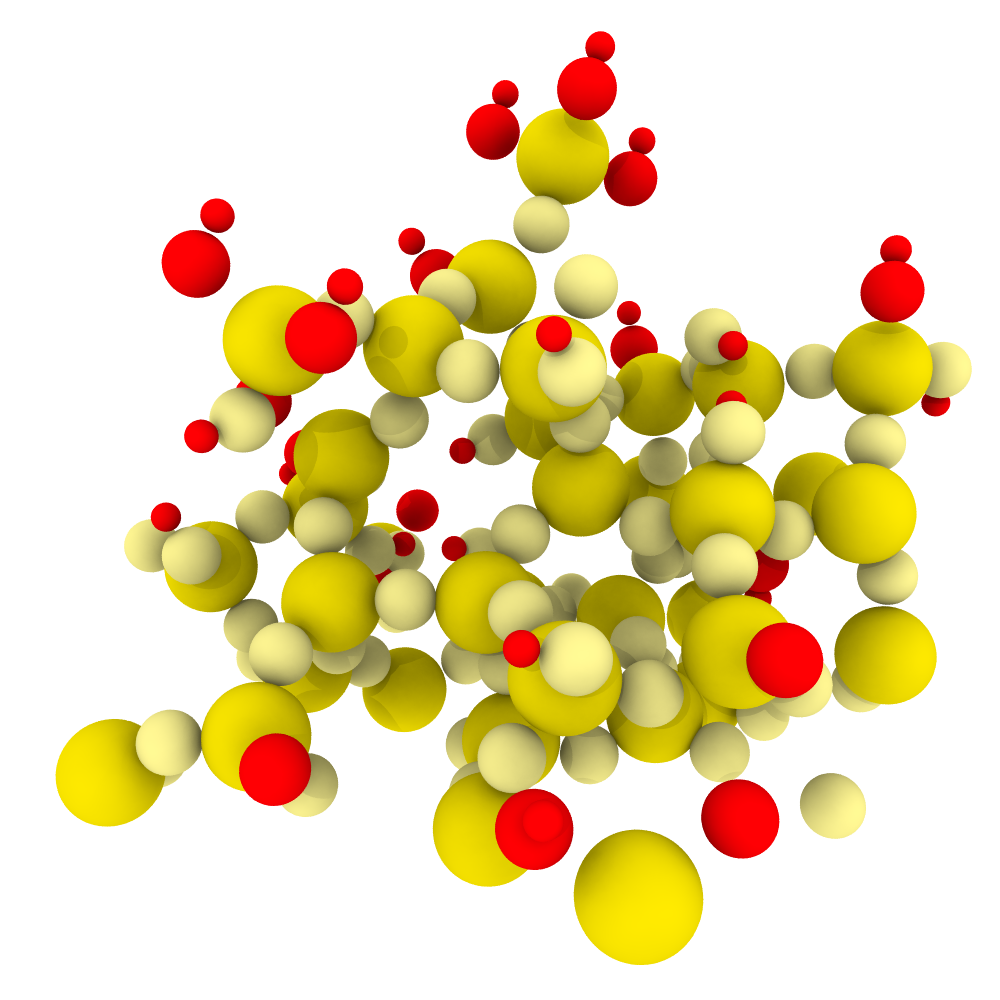
\includegraphics[width=0.7\textwidth]{images/passivation/passivation_example04.png}%
    \caption{
        Example of the result of the passivation procedure. Here the oxygen and hydrogen molecules are red, silicon atoms are yellow, and silicon-oxygen atoms are light yellow.%
    }%
    \label{fig:passivation_example}%
\end{figure}%

A good measure of the performance of the passivation method is the surface density of silanol after passivation. This number is often called the \emph{silanol number}, and us considered to be a physico-chemical constant, with a numerical value $\alpha_\text{OH} = 4.6$ (least-squares method) and $\alpha_\text{OH}\text{ nm}^{-2}$ (arithmical mean) \cite{zhuravlev1999silanol}, and is known in literature as the Kiselev-Zhuravlev constant. As we will see, measuring the surface area of porous system is not trivial, so estimating this density is not trivial. But by creating a completely flat pore and passivating it, we found that we got a silanol surface density between 4 and 7 nm$^{-2}$, depending on how we measure the surface area of the pore, and how we cound the number of silanol groups. % $\approx 7.05\text{ nm}^{-2}$ (if counting number of inserted hydrogen atoms) or $\approx 3.53\text{ nm}^{-2}$ (if counting number if inserted oxygen atoms). MAYBE MEASURE THIS PROPERLY?

% \todobo{Decide on whether to include silanol density stuff, and if so, write it}
% \orangebox{
% A good measure of the performance of the passivation method is the surface density of silanol after passivation. This number is often called the \emph{silanol number}, and us considered to be a physico-chemical constant, with a numerical value $\alpha_\text{OH} = 4.6$ (least-squares method) and $\alpha_\text{OH}\text{ nm}^{-2}$ (arithmical mean) \cite{zhuravlev1999silanol}, and is known in literature as the Kiselev-Zhuravlev constant. As we will see, measuring the surface area of porous system is not trivial, so estimating this density is not trivial. But by creating a completely flat pore and passivating it, we found that we created a silanol surface density of $\approx 7.05\text{ nm}^{-2}$ (if counting number of inserted hydrogen atoms) or $\approx 3.53\text{ nm}^{-2}$ (if counting number if inserted oxygen atoms). MAYBE MEASURE THIS PROPERLY?

% If the big number (7): since we inserted neutrally, the excess atoms will diffuse into the water anyway
% If the small number: the water we inject later will passivate the rest of the atoms
% Could also be caused by how we cut??
% The surface area is really bigger than $L^2$, since the atoms make a ``rough'' surface, not flat.
% }